\section{Event reconstruction and particle identification}
%%%%%%%%%%%%%%%%%%%%%%%%%%%%%%%%%%%%%%%%%%%%%%%%%%%%%%
\label{sec:Objects}

In CMS, the physics object reconstruction and identification is based on standard algorithms developed by the collaboration and used by all the physics analyses. In this section, the techniques used for the reconstruction and identification of the physics objects of interest for \hwwllnn analyses are described.

\subsection{The Particle Flow technique}

The Particle Flow (PF) event reconstruction technique~\cite{CMS-PAS-PFT-09-001} aims at the reconstruction and identification of all the stable particles in the event, i.e. electrons, muons, photons, charged and neutral hadrons, with a thorough combination of the information from all CMS sub-detectors, in order to determine their energy, direction and type. These individual particles are then used, for example, to build jets, to measure the missing transverse energy \MET, to reconstruct the $\tau$ from their decay products, to quantify the charged lepton isolation and to tag b-jets.

The CMS detector is well suited for this purpose. Indeed, the presence of a large internal silicon tracker immersed in an intense solenoidal magnetic field allows the reconstruction of charged particles with high efficiency and small fake rate, and provides a high precision measurement of the particle \pt down to about $150\,\MeV$, for $|\eta|\leq2.6$. The high granularity of the ECAL calorimeter is the additional key element for the feasibility of the PF technique, allowing the reconstruction of photons and electrons with high energy resolution.

The first step of the PF technique consists in the reconstruction of the basic elements from the various sub-detectors, such as charged-particle tracks, calorimeter clusters and muon tracks. These elements, which are provided by the sub-detectors with high efficiency an low fake rate, are then connected together with a link algorithm.

The good performance of the tracking system are achieved by means of an iterative tracking strategy~\cite{Chatrchyan:2014fea}, based on the Kalman Filter algorithm~\cite{Billoir:1990we}. The basic idea of iterative tracking is that initial iterations search for tracks that are easiest to find, e.g. high \pt tracks produced near the interaction region. After each iteration, hits associated to reconstructed tracks are removed from the hit collection, thereby reducing the combinatorial complexity and simplifying the subsequent iterations, which aim at finding more complicated set of tracks, e.g. low \pt or displaced tracks. The \emph{Iteration 0}, where the majority of tracks are reconstructed, is designed to identify prompt tracks with $\pt>0.8$\,\GeV that have three hits in the three layers of the pixel detector. \emph{Iteration 1} is used to recover prompt tracks that have only two pixel hits. \emph{Iteration 2} aims at finding low-\pt prompt tracks while \emph{Iterations 3--5} are intended to find tracks that originate outside the collision point, i.e. tracks produced by a secondary vertex, and to recover undetected tracks in the previous iterations. Each iteration proceeds according to four steps:
\begin{itemize}
\item \emph{seeding}: initial track candidates are obtained using 2 or 3 hits in the innermost layers (these proto-tracks are called seeds);
\item \emph{pattern recognition}: this step is based on Kalman Filter and searches for hits in the outer layers that could be associated to the initial track candidate, reconstructing the particle trajectory;
\item \emph{track fitting}: in this step a fit of the trajectory is performed, using its associated hits and providing an estimate of the track parameters (\pt, $\eta$, $\phi$, charge, etc.);
\item \emph{selection}: finally tracks are selected based on quality requirements.
\end{itemize}

The high detection efficiency of the calorimeters is based on a specific calorimeter clustering algorithm, which is performed separately in each sub-detector. The algorithm is based on three steps: in the first step, ``cluster seeds'' are identified as local calorimeter cells with an energy deposit above a given threshold. Then, ``topological clusters'' are grown from the seeds by gathering cells with at least one side in common with a cell already in the cluster, and with an energy above a given threshold. A topological cluster usually gives rise to many ``particle flow clusters'' as seeds, which are identified sharing the energy of each cell among the particle flow clusters, thereby allowing the determination of the particle flow cluster energy and position.

These elements are then connected to each other using a link algorithm, which identifies blocks of elements that are topologically compatible. For example, a charged-particle track is linked to a calorimeter particle flow cluster if the extrapolated position from the track to the calorimeter is compatible with the cluster boundaries. From these blocks, PF candidates are identified according to the following order:
\begin{itemize}
\item Muons: a \emph{global muon} gives rise to a \emph{PF muon} if its combined \pt measurement is compatible within 3 standard deviation with the one provided by the sole tracker. The corresponding track is removed from the block;
\item Electrons: electrons tend to give rise to short tracks, and to lose energy by Bremsstrahlung in the tracker layers on their way to the calorimeter. The link between a charged-particle track (refitted with the Gaussian-Sum Filter~\cite{Adam:815410}) and one or more ECAL clusters identifies a \emph{PF electron}. After the identification, the corresponding tracks and clusters are removed from the block.
\item Charged hadrons: the remaining tracks give rise to \emph{PF charged hadrons}. Tracks can be linked to ECAL and HCAL clusters, and the energy is determined taking into account information from calorimeters;
\item Photons and neutral hadrons: ECAL clusters not linked with tracks give rise to \emph{PF photons}, while the remaining HCAL clusters are identified as \emph{PF neutral hadrons}.
\end{itemize}
After the identification of all PF candidates in the event, \emph{PF jets} are clustered as described in Sec.~\ref{chap2:jets}. The last step is the reconstruction of the \emph{PF \ptmiss}, which is given by:

\begin{equation} 
\ptmiss = - \sum_{\mathrm{PF\,obj}} \vec{p}_\mathrm{T}^\mathrm{\,PF\,obj} \quad,
\end{equation}

where the sum extends over all the PF objects. The \MET is defined as the modulus of \ptmiss.

\subsection{Leptons reconstruction and identification}

\subsubsection{Muons}
Muons produced at the collision point can go through the entire detector with a negligible energy loss, thus reaching the detector outermost part where the muon chambers are installed (see Sec.~\ref{sec:muonsyst}). Muons interact through ionization with the layers of the silicon tracker, which is able to reconstruct their tracks (\emph{tracker track}). The muon tracks are also reconstructed using the muon system (\emph{standalone muon track}). Based on these objects, two reconstruction approaches are used: in the first method (outside-in), for each standalone muon tracks a tracker track is searched for by extrapolating the two tracks to a common surface. If a match is found, the hits associated to the two tracks are fitted together giving rise to a \emph{Global Muon}. The second approach (inside-out) consists in considering all tracker tracks with $\pt > 0.5$\,\GeV as potential muon candidates and are extrapolated to the muon system taking into account the magnetic field, the expected energy losses and the multiple scattering in the detector material. If at least one muon segment (a short track stub made of DT or CSC hits) matches the extrapolated tracks, the corresponding tracker track is identified as a \emph{Tracker Muon}.

The matching with the muon system improves significantly the muon \pt resolution that can be obtained from the tracker only, especially in the region with $\pt > 200$\GeV, as shown in Fig.~\ref{fig:muptres}.
\begin{figure}[htb]
\centering
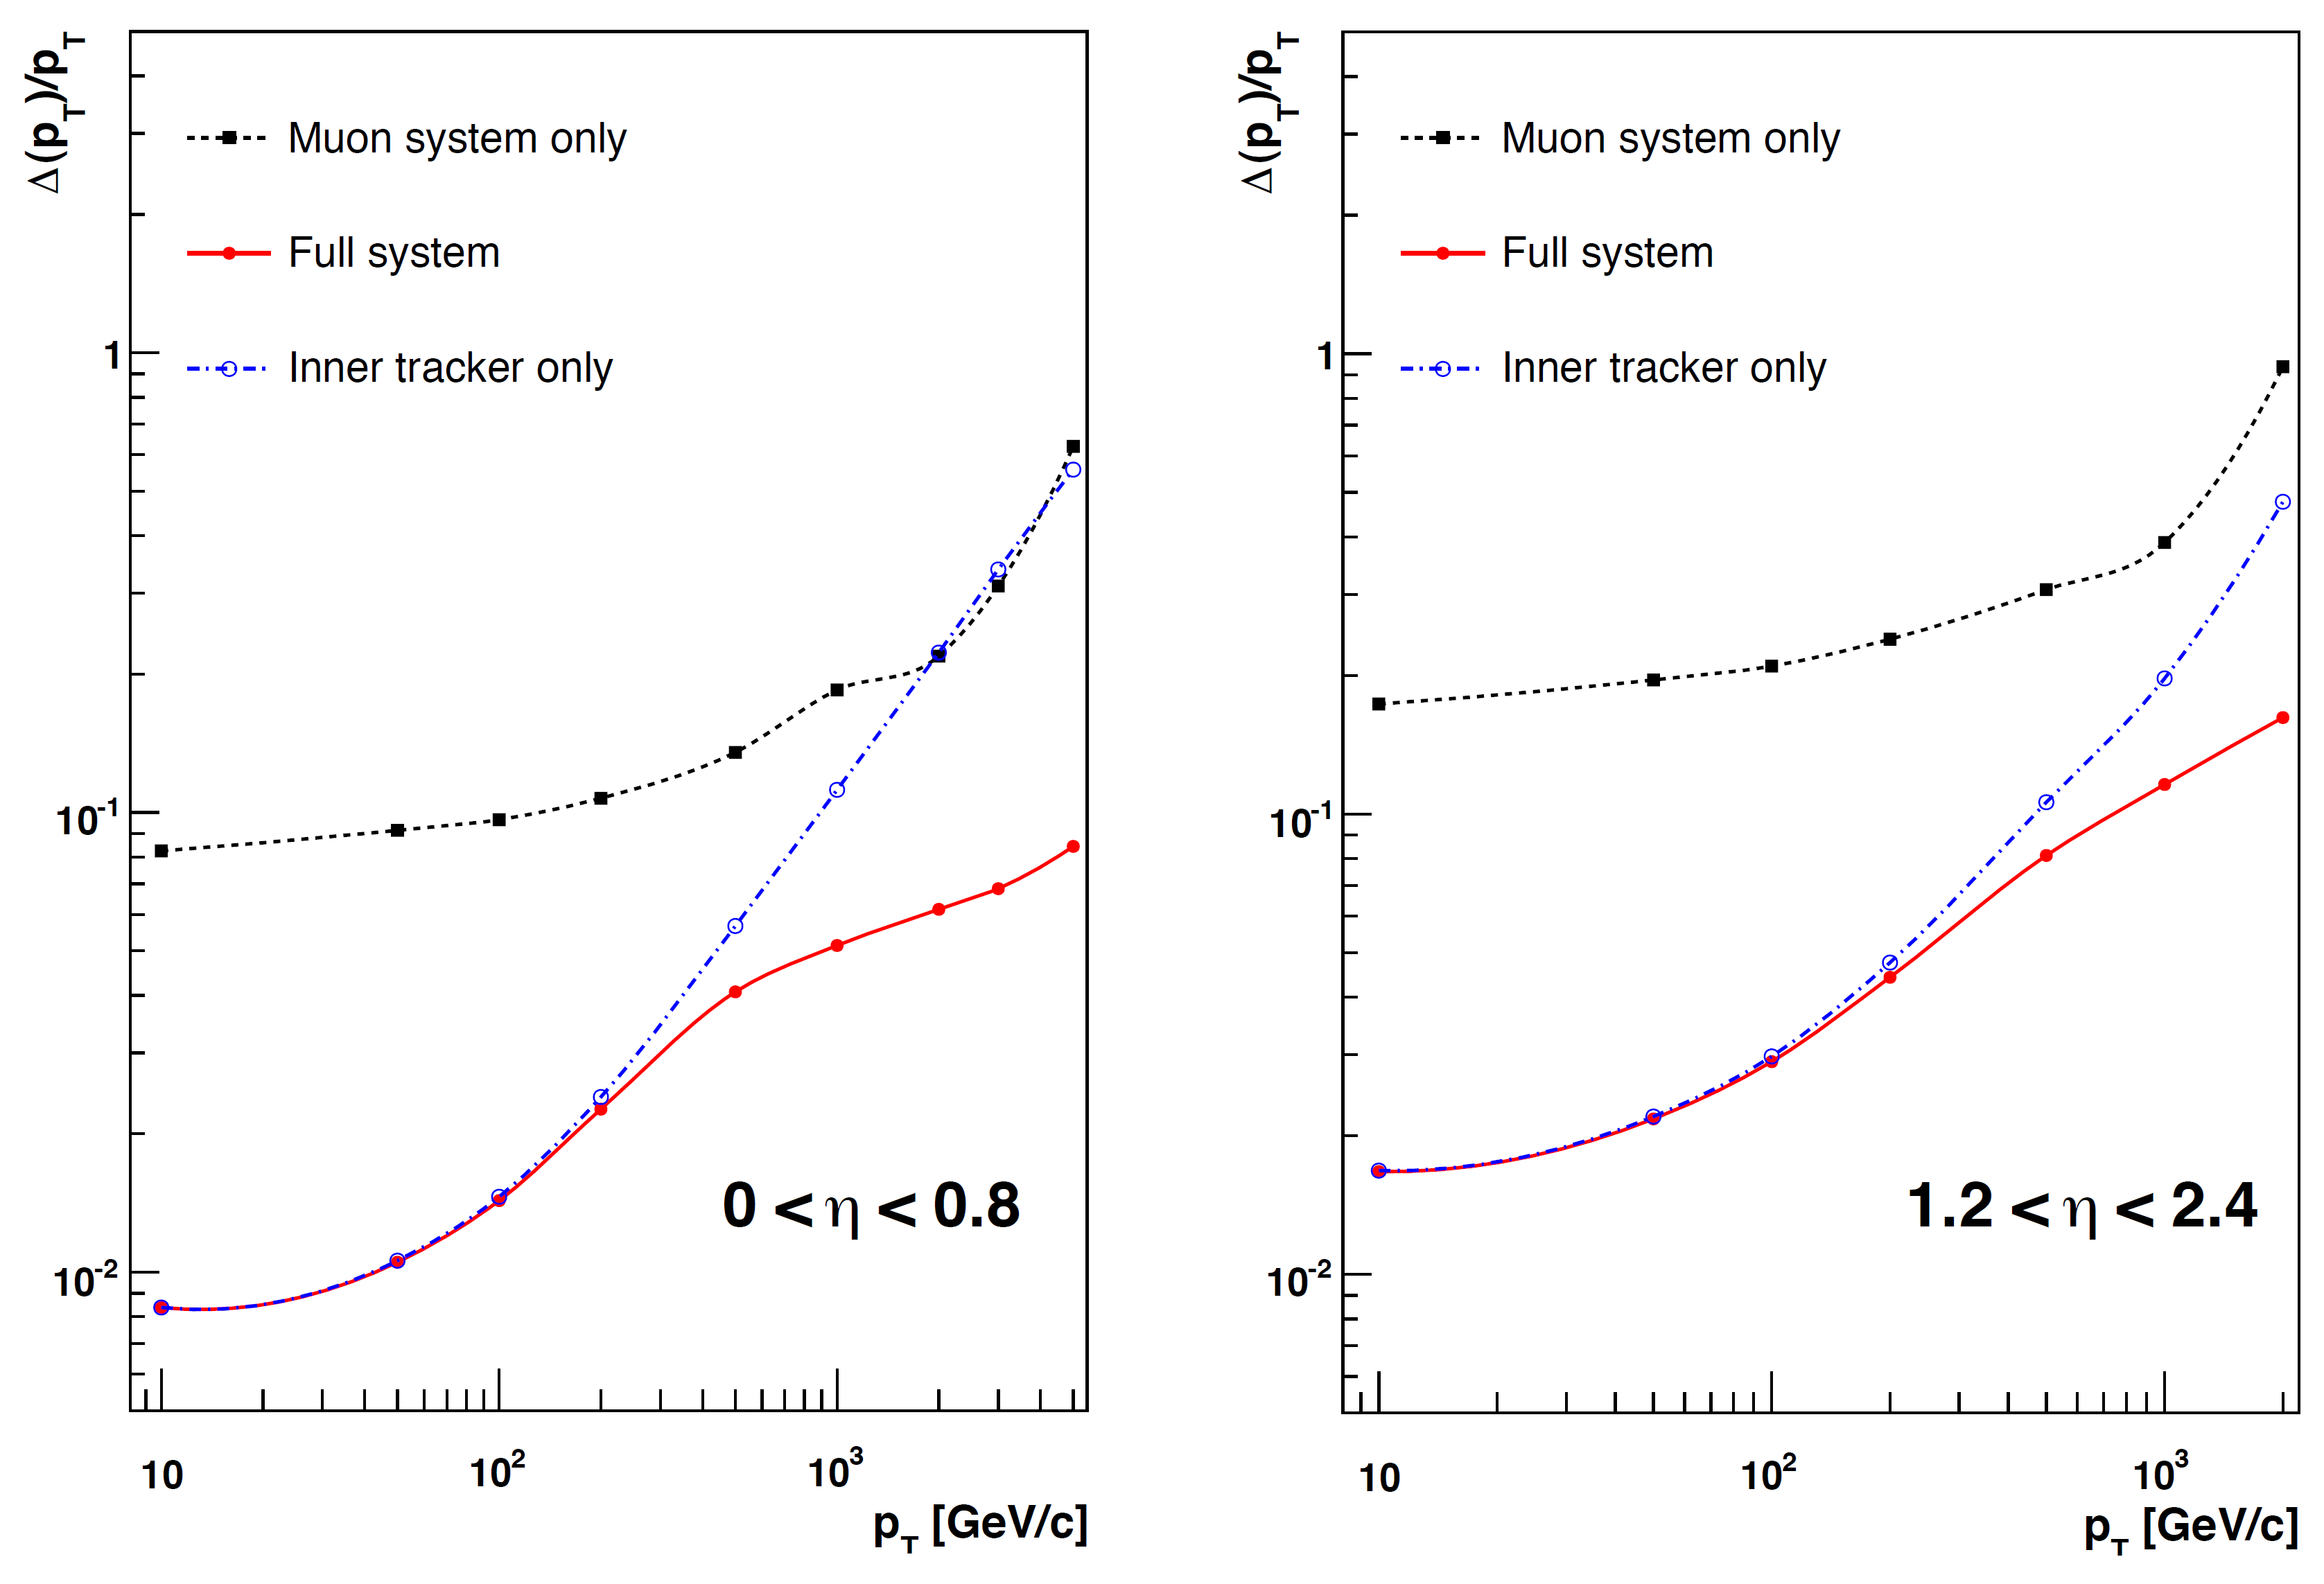
\includegraphics[width=0.6\textwidth]{images/muptres.png}
\caption{Muon \pt resolution as a function of the muon \pt in the barrel (left) and in the endcap (right) regions. The resolution is provided for the measurement using the tracking system or the muon system only, as well as for the combination of the two methods.}\label{fig:muptrese}
\end{figure}
\subsubsection{Electrons}
	

	
\subsection{Jets reconstruction and identification}\label{chap2:jets}

	\subsubsection{Jet b tagging}
